\section{Практическое исследование компиляционного синтеза}

\subsection{Задание 3.3.1. Формирование фонетической базы}

Фонетическая база сформирована из записей лабораторной работы №1: гласные
[а], [о], [у], [э], [ы], [и] вырезаны из \texttt{sample1.wav}, [й] --- из
\texttt{sample1b.wav}, [д] --- из слога <<да>> (\texttt{sample5.wav}).
Согласные [л], [р], [п], [т] отсутствовали в записях первой работы, поэтому
они вырезаны из слогов <<ла>>, <<ра>>, <<па>>, <<ты>>, записанных для
задания 3.3.5; из слога <<ма>> вырезан более чистый носовой [м] (в
\texttt{sample4.wav} он был перегружен по уровню). Границы фонем
размечались вручную по осциллограммам и спектрограммам. Всего получено
13 фонем; их характеристики приведены в таблице~\ref{tab:base},
осциллограммы --- на рисунке~\ref{fig:base}.

\begin{table}[H]
	\centering
	\small
	\caption{Фонетическая база (задание 3.3.1)}
	\label{tab:base}
	\begin{tabular}{|l|l|l|l|l|l|}
		\hline
		Фонема & Источник & Длит., с & $F_0$, Гц & Пик, дБFS & RMS, дБFS \\
		\hline
		[а] & \texttt{sample1} & 0,24 & 119 & $-21{,}4$ & $-29{,}0$ \\
		\hline
		[о] & \texttt{sample1} & 0,24 & 145 & $-14{,}3$ & $-23{,}2$ \\
		\hline
		[у] & \texttt{sample1} & 0,24 & 172 & $-15{,}3$ & $-21{,}7$ \\
		\hline
		[э] & \texttt{sample1} & 0,24 & 188 & $-16{,}6$ & $-25{,}3$ \\
		\hline
		[ы] & \texttt{sample1} & 0,24 & 205 & $-18{,}1$ & $-26{,}3$ \\
		\hline
		[и] & \texttt{sample1} & 0,24 & 205 & $-19{,}5$ & $-26{,}9$ \\
		\hline
		[м] & слог <<ма>> & 0,10 & 136 & $-24{,}2$ & $-32{,}9$ \\
		\hline
		[й] & \texttt{sample1b} & 0,12 & 119 & $-24{,}7$ & $-33{,}1$ \\
		\hline
		[л] & слог <<ла>> & 0,15 & 129 & $-23{,}8$ & $-33{,}9$ \\
		\hline
		[р] & слог <<ра>> & 0,10 & 126 & $-16{,}8$ & $-29{,}2$ \\
		\hline
		[п] & слог <<па>> & 0,06 & 133 & $-14{,}2$ & $-30{,}3$ \\
		\hline
		[т] & слог <<ты>> & 0,06 & --- & $-24{,}0$ & $-34{,}5$ \\
		\hline
		[д] & слог <<да>> & 0,08 & 124 & $-17{,}0$ & $-24{,}4$ \\
		\hline
	\end{tabular}
\end{table}

\begin{figure}[H]
	\centering
	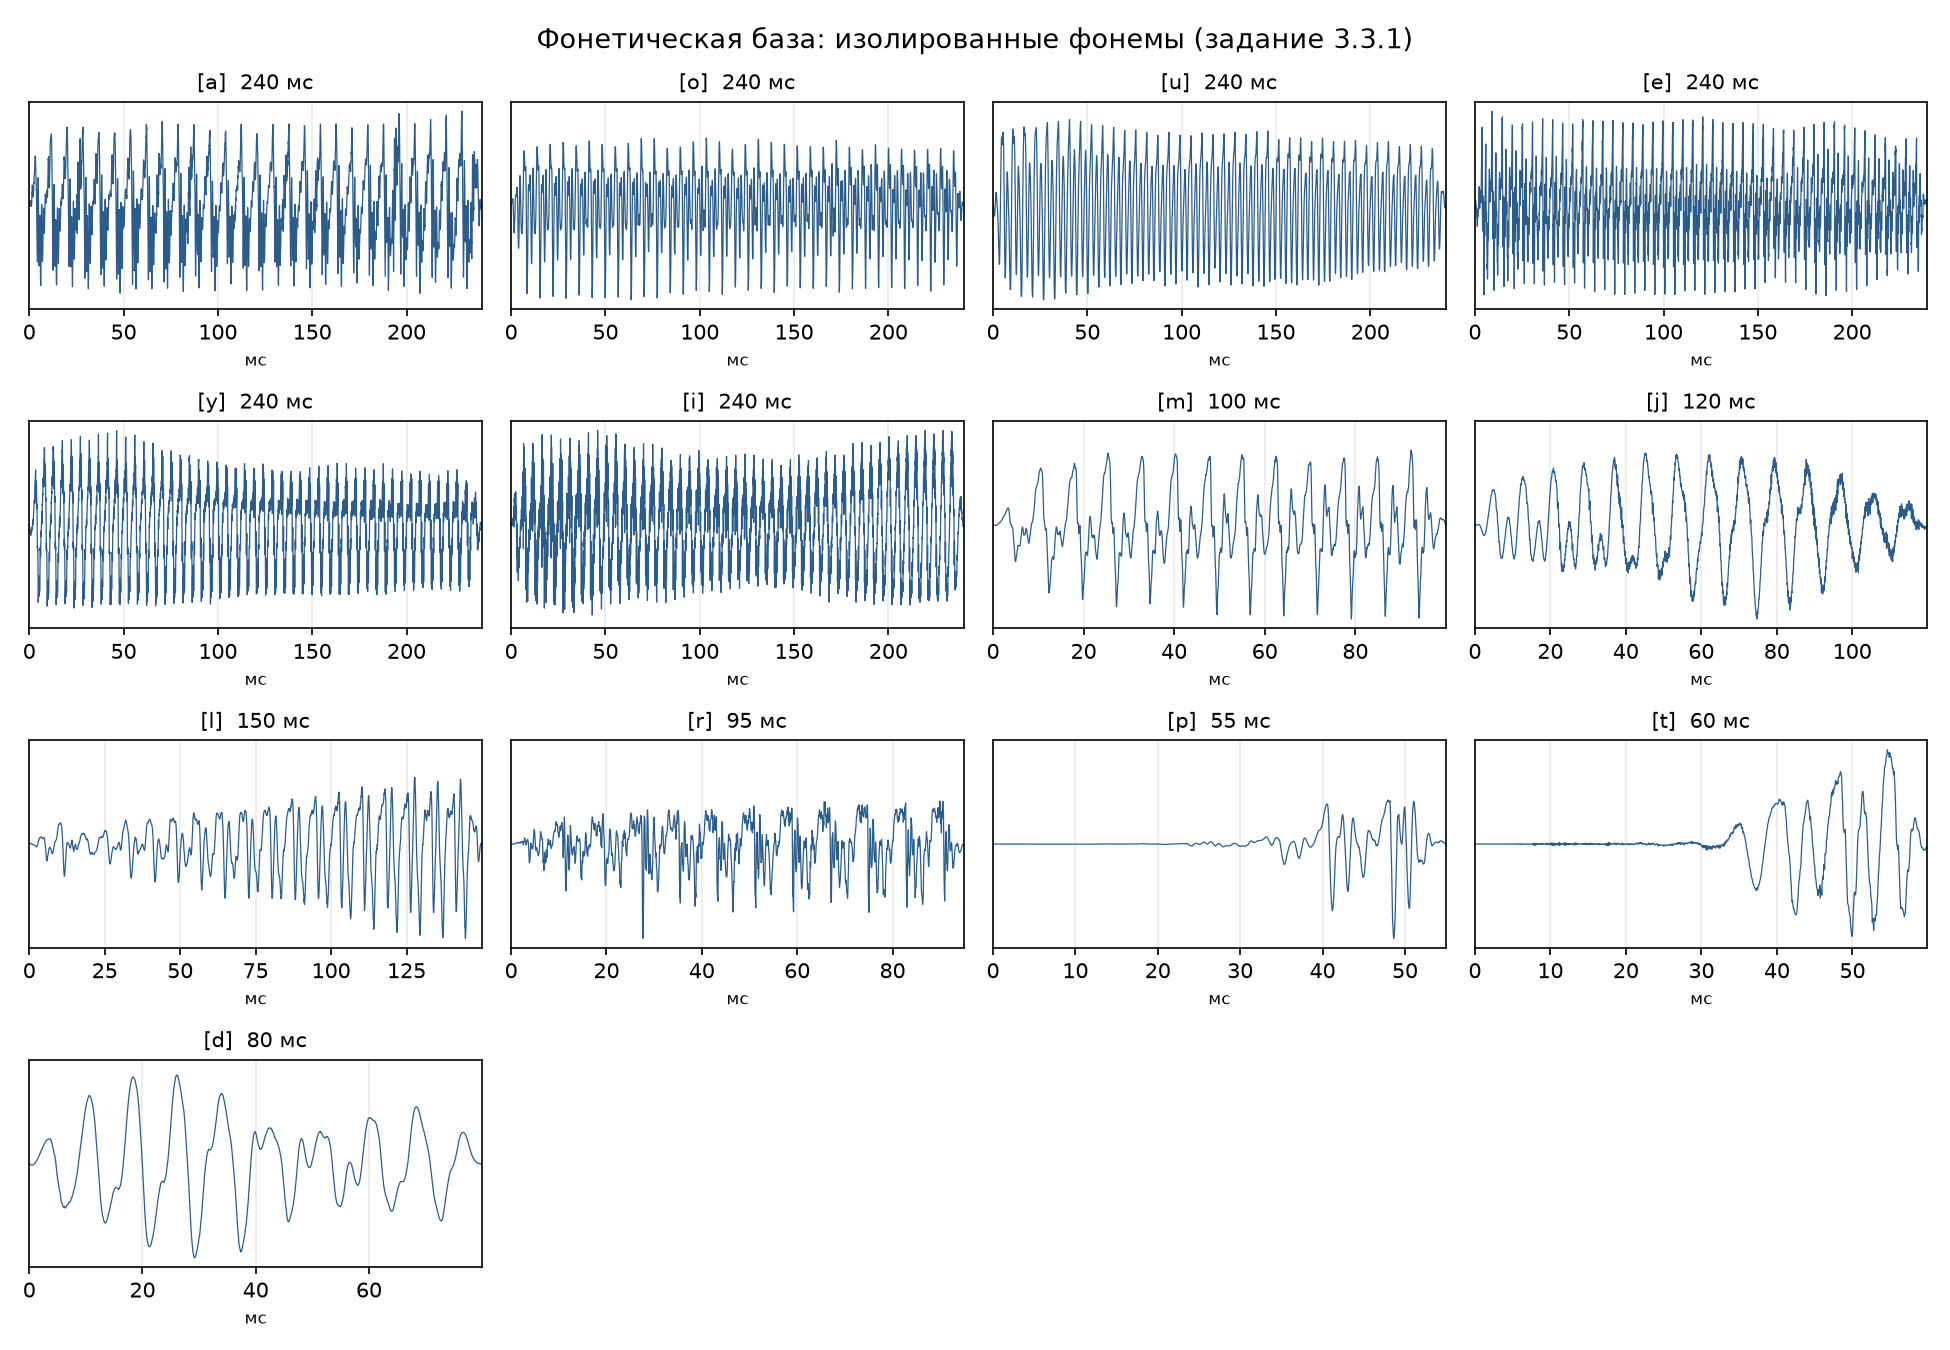
\includegraphics[width=\textwidth]{lab3_phoneme_base.png}
	\caption{Осциллограммы фонем фонетической базы}
	\label{fig:base}
\end{figure}

Обращает на себя внимание различие частоты основного тона гласных,
записанных в лабораторной работе №1: от 119~Гц ([а]) до 205~Гц ([ы], [и]).
Это связано с тем, что гласные произносились в виде перечисления, и тон
заметно повышался к концу списка. Данное обстоятельство впоследствии
оказывается главным источником искажений при компиляции.

\subsection{Задание 3.3.2. Компиляция фраз из фонем}

По фонемным текстам из раздела 3.2 созданы четыре фразы. Каждая фонема
бралась из базы, обрезалась до типовой длительности своего класса и
приводилась к типовому уровню, после чего сегменты склеивались с плавными
фронтами (3~мс). Просодика (ударение, мелодика) на этом этапе специально не
задавалась. Использованные параметры сегментов приведены в
таблице~\ref{tab:segparams}.

\begin{table}[H]
	\centering
	\small
	\caption{Типовые длительности и уровни сегментов}
	\label{tab:segparams}
	\begin{tabular}{|l|c|c|}
		\hline
		Класс сегмента & Длительность, мс & Уровень (критерий, дБFS) \\
		\hline
		ударный гласный & 220 (170) & RMS $-18$ \\
		\hline
		безударный гласный & 160 (120) & RMS $-18$ \\
		\hline
		сонорный [м л р] & 90 / 90 / 65 & RMS $-23$ \\
		\hline
		[й] & 60 & RMS $-24$ \\
		\hline
		взрывные [п т д] & 70 & пик $-15$ / $-15$ / $-12$ \\
		\hline
	\end{tabular}
\end{table}

В скобках указаны длительности для коротких фраз <<Ты дома?>> и
<<Ты дома.>>. Результаты компиляции четырёх фраз сведены в
таблицу~\ref{tab:phonemes}. В качестве примера в
таблице~\ref{tab:phrase1} приведена последовательность сегментов фразы
<<Мама мыла раму.>> с их параметрами.

\begin{table}[H]
	\centering
	\small
	\caption{Параметры фраз, скомпилированных из фонем}
	\label{tab:phonemes}
	\begin{tabular}{|l|c|c|c|c|}
		\hline
		Фраза & Длит., с & $F_0$ мед., Гц &
		$F_0$ мин.--макс., Гц & Скачок $F_0$, Гц \\
		\hline
		<<Мама мыла раму.>> & 1,92 & 120 & 103--172 & 35 \\
		\hline
		<<Мама, папа и я.>> & 2,31 & 119 & 105--205 & 100 \\
		\hline
		<<Ты дома?>> & 0,71 & 126 & 103--145 & 35 \\
		\hline
		<<Ты дома.>> & 0,71 & 126 & 103--145 & 35 \\
		\hline
	\end{tabular}
\end{table}

\begin{table}[H]
	\centering
	\small
	\caption{Последовательность сегментов фразы <<Мама мыла раму.>>}
	\label{tab:phrase1}
	\begin{tabular}{|l|c|c|c|}
		\hline
		Фонема & Класс & Длит., с & $F_0$, Гц \\
		\hline
		{[м]} & сонорный & 0,090 & 136 \\
		{[а]} & ударный & 0,220 & 119 \\
		{[м]} & сонорный & 0,090 & 136 \\
		{[а]} & безударный & 0,160 & 119 \\
		{[м]} & сонорный & 0,090 & 136 \\
		{[ы]} & ударный & 0,220 & 205 \\
		{[л]} & сонорный & 0,090 & 129 \\
		{[а]} & безударный & 0,160 & 119 \\
		{[р]} & сонорный & 0,065 & 126 \\
		{[а]} & ударный & 0,220 & 119 \\
		{[м]} & сонорный & 0,090 & 136 \\
		{[у]} & ударный & 0,220 & 172 \\
		\hline
	\end{tabular}
\end{table}

Из таблицы~\ref{tab:phrase1} виден главный дефект фонемной компиляции:
частоты основного тона соседних фонем сильно различаются ([а] --- 119~Гц,
[ы] --- 205~Гц, [у] --- 172~Гц), поскольку изолированные гласные были
произнесены с восходящей интонацией списка. На стыках фонем возникают
скачки $F_0$ до 35~Гц, а в фразе с [и] и [й] --- до 100~Гц.

\subsection{Задание 3.3.3. Анализ скомпилированной речи}

Прослушивание скомпилированных фраз и их сравнение с эталонами
(таблица~\ref{tab:compare}, рис.~\ref{fig:wave},~\ref{fig:f0}) позволило
выделить положительные и отрицательные стороны компиляционного метода.

\begin{table}[H]
	\centering
	\footnotesize
	\caption{Сравнение эталонных и синтезированных фраз}
	\label{tab:compare}
	\begin{tabular}{|l|l|c|c|c|}
		\hline
		Фраза & Вариант & Длит., с & $F_0$ мед., Гц & $F_0$ мин.--макс., Гц \\
		\hline
		\multirow{3}{*}{<<Мама мыла раму.>>} & эталон & 2,17 & 136 & 99--190 \\
		\cline{2-5}
		& фонемы & 1,92 & 120 & 103--172 \\
		\cline{2-5}
		& слоги & 1,90 & 134 & 121--145 \\
		\hline
		\multirow{3}{*}{<<Мама, папа и я.>>} & эталон & 3,07 & 127 & 98--147 \\
		\cline{2-5}
		& фонемы & 2,31 & 119 & 105--205 \\
		\cline{2-5}
		& слоги & 2,31 & 133 & 113--143 \\
		\hline
		\multirow{3}{*}{<<Ты дома?>>} & эталон & 0,61 & 128 & 118--216 \\
		\cline{2-5}
		& фонемы & 0,71 & 126 & 103--145 \\
		\cline{2-5}
		& слоги & 0,87 & 133 & 119--143 \\
		\hline
		\multirow{3}{*}{<<Ты дома.>>} & эталон & 0,52 & 132 & 108--145 \\
		\cline{2-5}
		& фонемы & 0,71 & 126 & 103--145 \\
		\cline{2-5}
		& слоги & 0,87 & 133 & 119--143 \\
		\hline
	\end{tabular}
\end{table}

\begin{figure}[H]
	\centering
	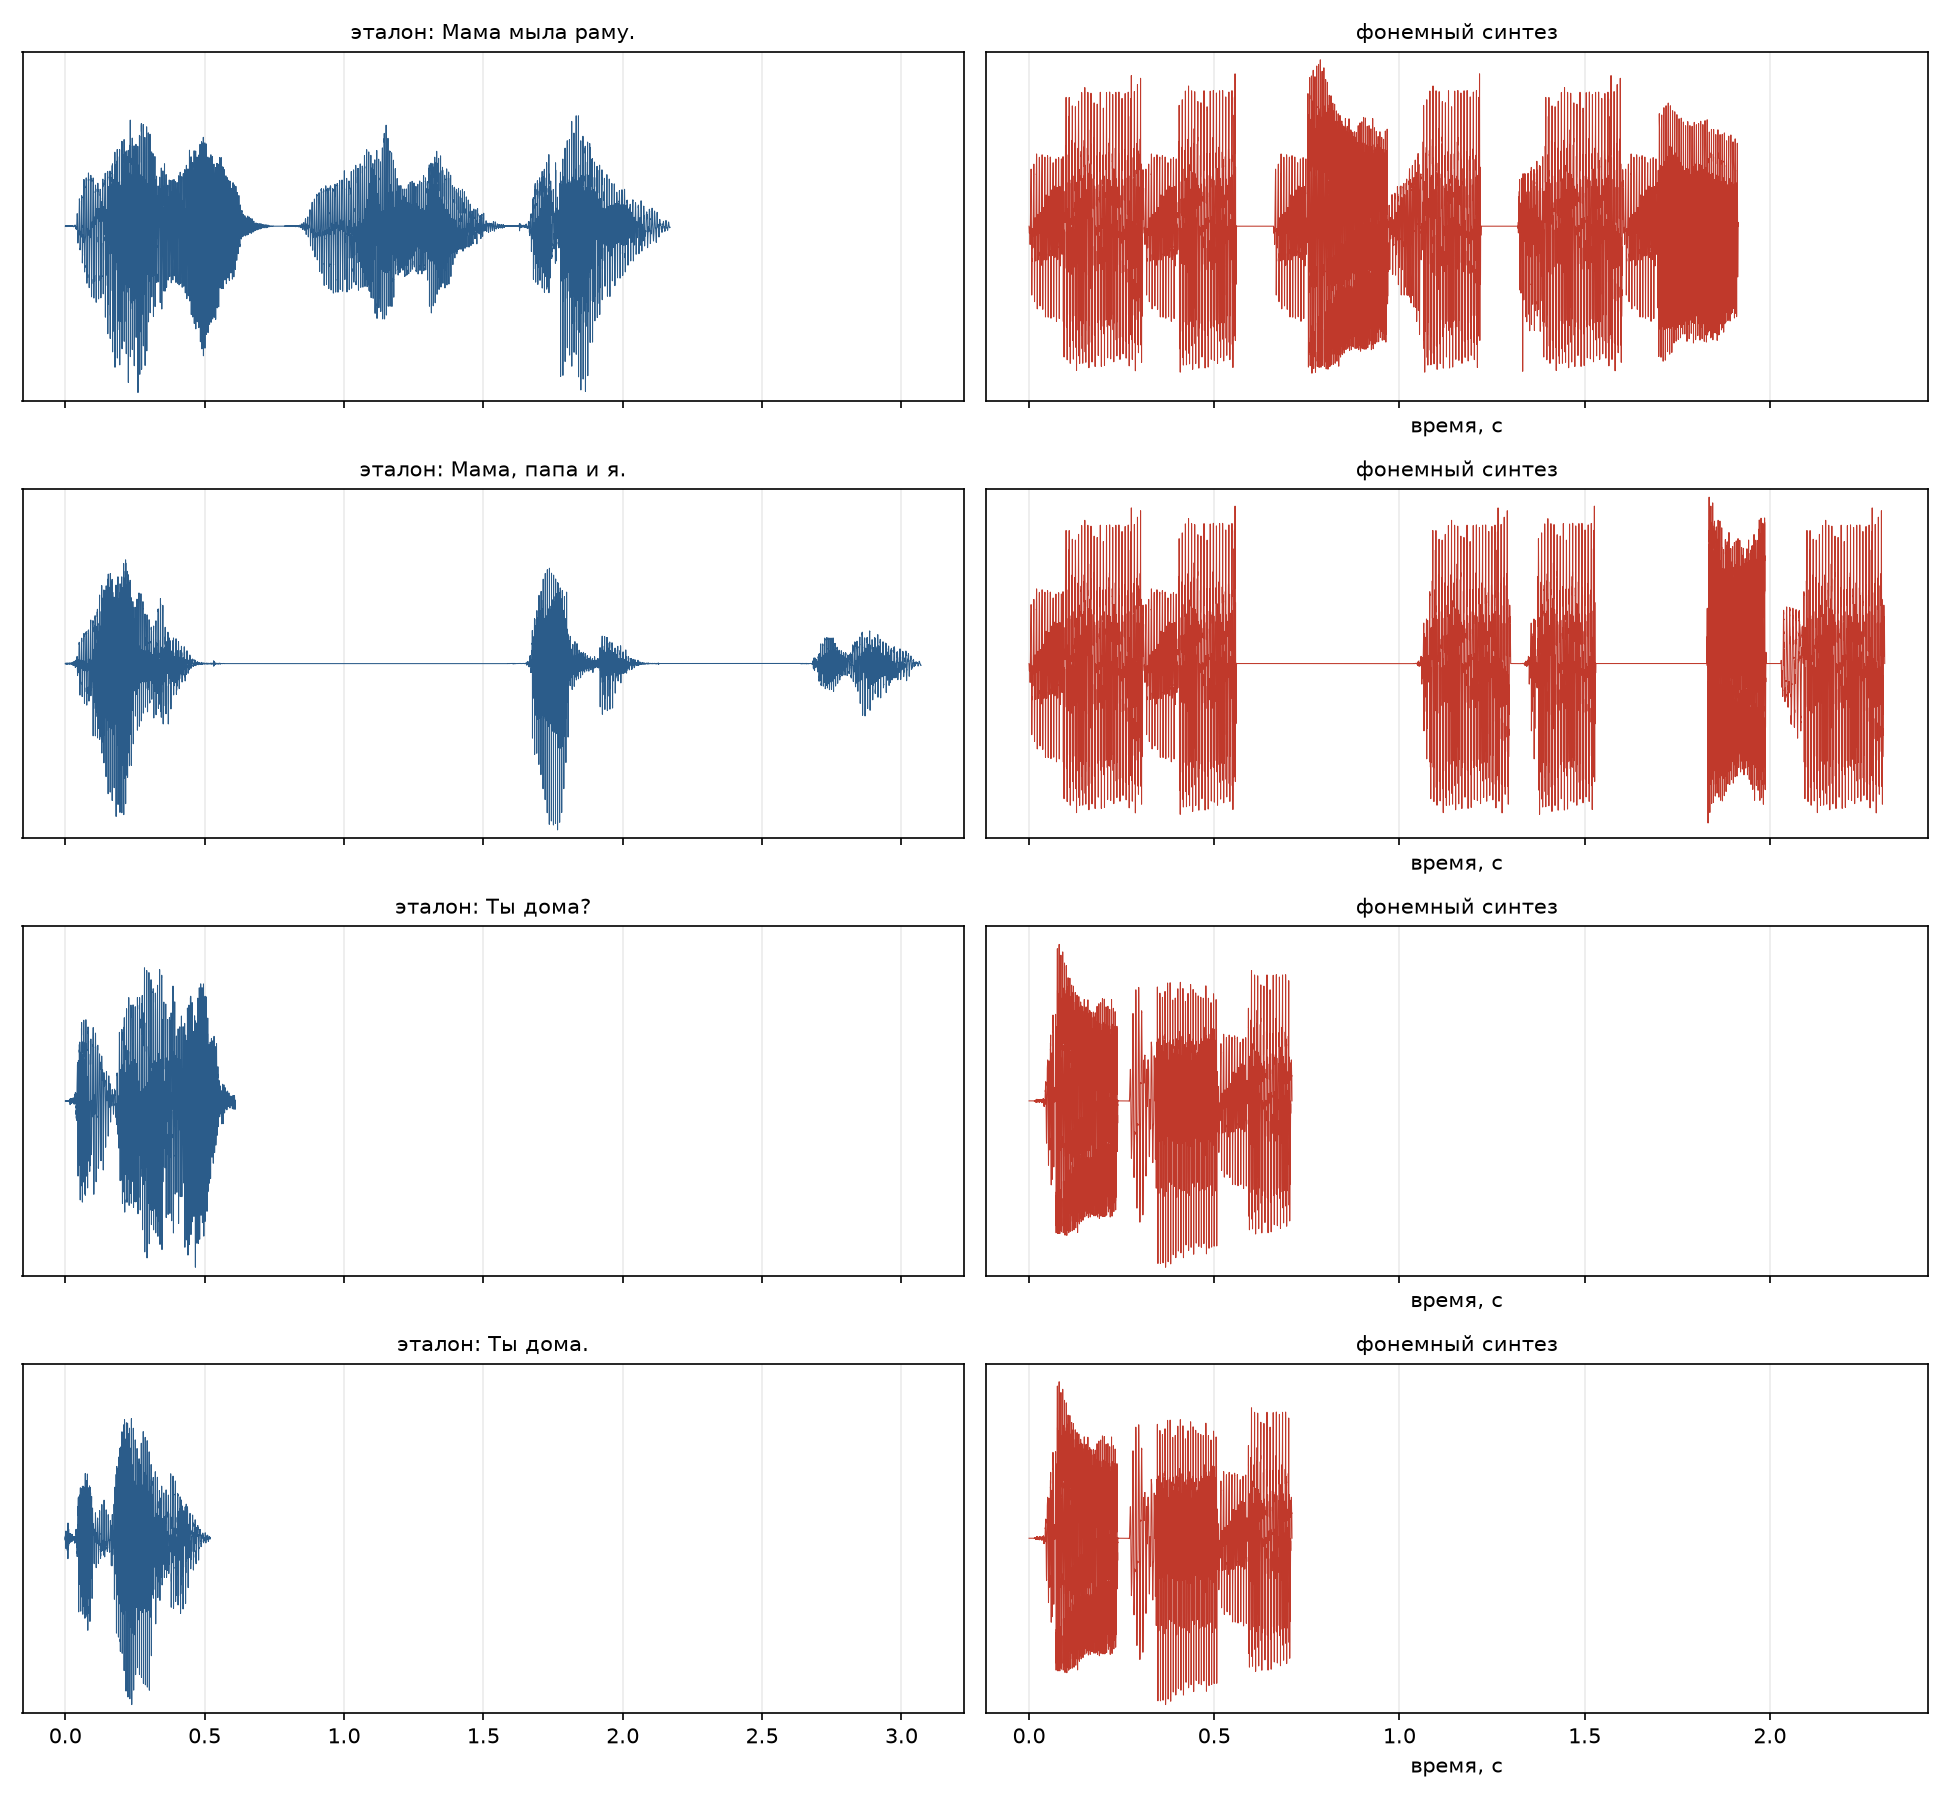
\includegraphics[width=\textwidth]{lab3_wave_compare.png}
	\caption{Осциллограммы эталонных фраз и фраз, скомпилированных из фонем}
	\label{fig:wave}
\end{figure}

\begin{figure}[H]
	\centering
	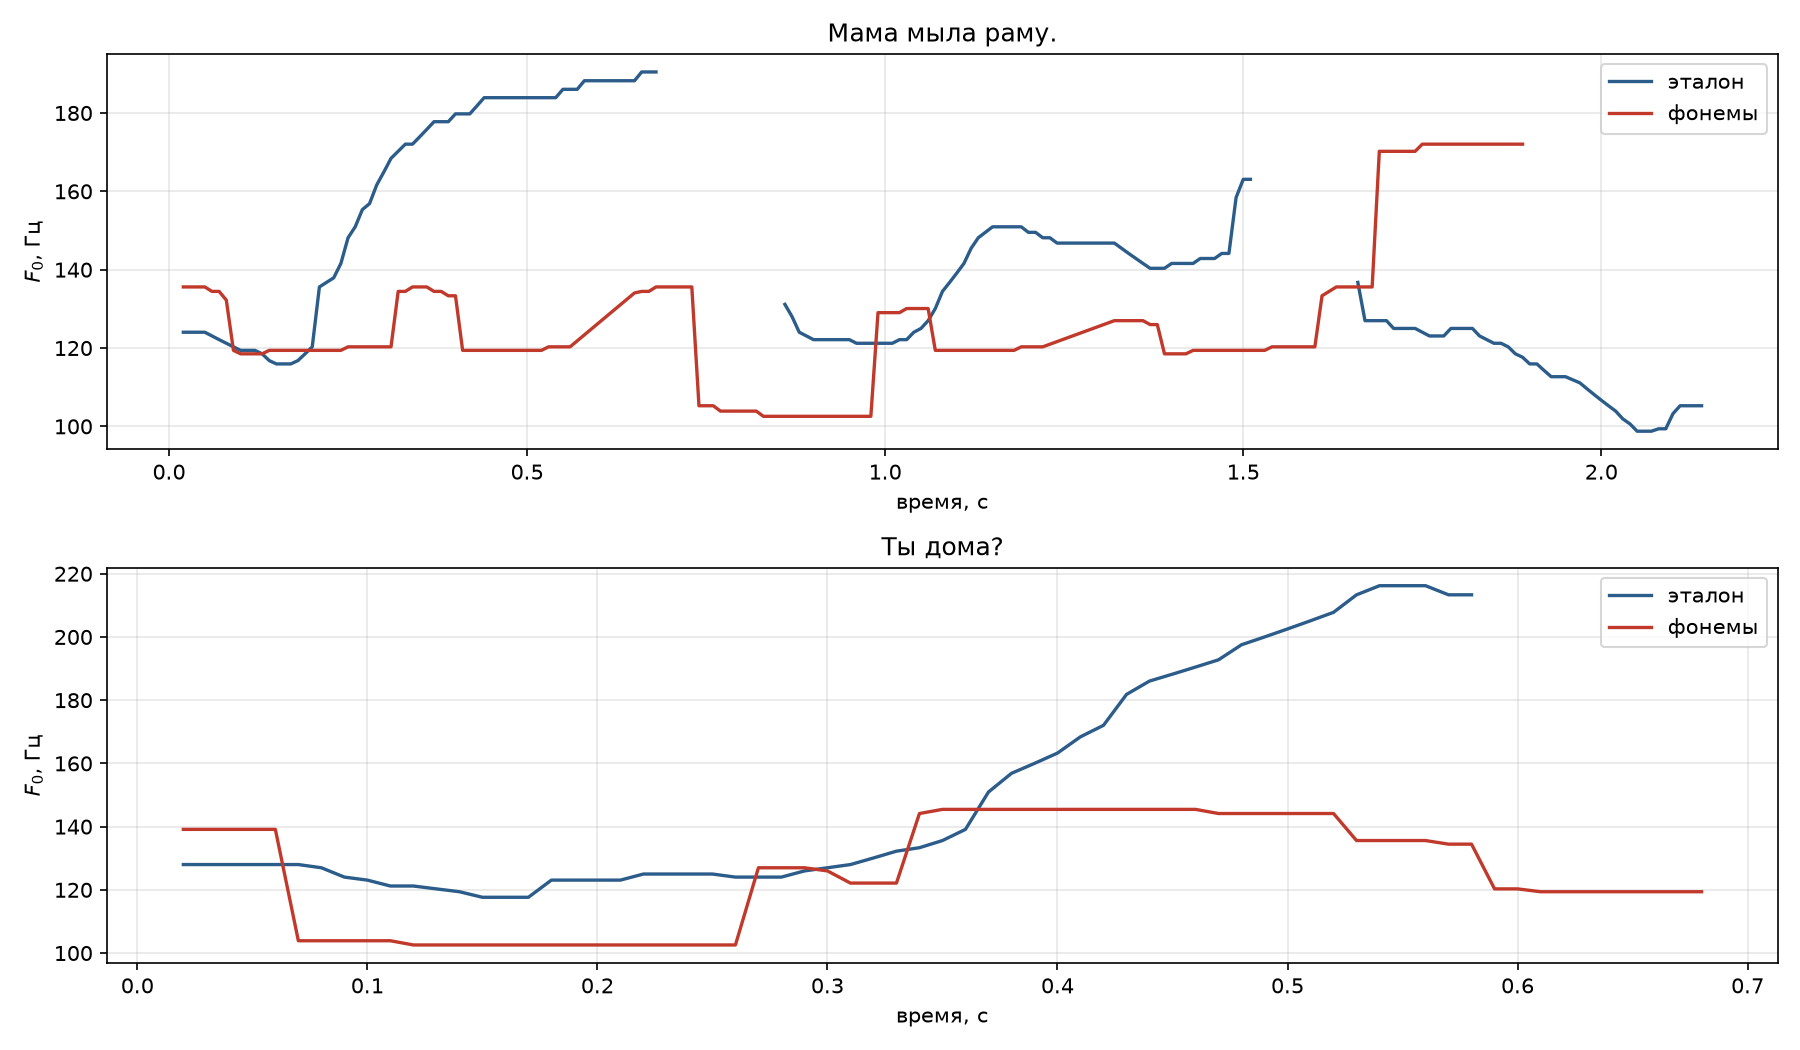
\includegraphics[width=\textwidth]{lab3_f0_compare.png}
	\caption{Контуры $F_0$ эталонной и скомпилированной фразы}
	\label{fig:f0}
\end{figure}

\emph{Достоинства} компиляционного метода:
\begin{itemize}
	\item фразы разборчивы, все слова опознаются на слух;
	\item каждая фонема звучит естественно, поскольку взята из реальной
	речи;
	\item метод прост в реализации и не требует модели речеобразования.
\end{itemize}

\emph{Недостатки}, проявившиеся в нашем эксперименте:
\begin{itemize}
	\item из-за разного тона изолированных гласных на стыках фонем
	возникают скачки $F_0$ до 35--100~Гц, что воспринимается как
	<<скачущий>> голос;
	\item скомпилированные фразы почти монотонны: отсутствует мелодический
	контур, поэтому вопрос <<Ты дома?>> не отличим от утверждения
	<<Ты дома.>> (обе фразы собраны из одинаковых фонем);
	\item длительность синтезированных фраз меньше эталонной (ударные
	гласные взяты без удлинения), а средний уровень выше эталонного из-за
	нормировки всего файла;
	\item переходы между фонемами (коартикуляция) отсутствуют, что заметно
	на стыках согласных и гласных.
\end{itemize}
